\glsresetall
\chapter{State of the Art}
\label{chap:state_of_the_art}

In this chapter, we discuss the core concepts regarding the project, related work and the most modern techniques and available technology for the purpose today. All the information that will be presented was the result of a work of investigation through published articles, knowledge exchange and web searching.

The main purpose of the section \ref{sec:concepts} - \nameref{sec:concepts} is to introduce and provide a brief explanation about the core concepts. In the second section \ref{sec:related_work} - \nameref{sec:related_work} some published articles and posts of related work are presented. In the final section \ref{sec:technologies} - \nameref{sec:technologies}, all the important technologies are analysed and discussed using tables, diagrams and plain text.

\section{Concepts}
\label{sec:concepts}

The following concepts represents the baseline to understand the work related to this project.

\subsection{Microservices}
\label{subsec:microservices}

Microservices is ``an architectural style that structures an application as a collection of loosely coupled services, which implement business capabilities''\cite{microservices_definition}.

This kind of style has a very long history, and has being introduced and evolving since the first contact with topics like distributed computing, \gls{api} and containers.

The core concept of microservices stands in isolation, or by other words, what everyone wants to achieve when building a software with microservices in mind, is to share less things between the services and deal with correlated failures. In this sense, a service is a small part of the entire system (e.g. Get messages microservice), and represents a tiny feature of the whole service (e.g. Chat Service). To do this, normally every microservice is encapsulated inside a container (e.g. Docker container\cite{docker}), and each runs in its own process and communicates with the other using lightweight mechanisms, often an \gls{http} resource \gls{api}. ``A container is a standard unit of software that packages up code and all its dependencies so the application runs quickly and reliably from one computing environment to another''\cite{what_is_containers}.

On the other side, and for comparison purposes, we have another very well known architectural style, the monolithic. This style has a logically modular architecture, and the services are packaged and deployed in a single  application using a single code base. To compare both architectural styles presented before we have the figure \ref{fig:monolithic_and_microservices} that shows and provides a more clear insight about the differences between them.

\begin{figure}[H]
    \centering
    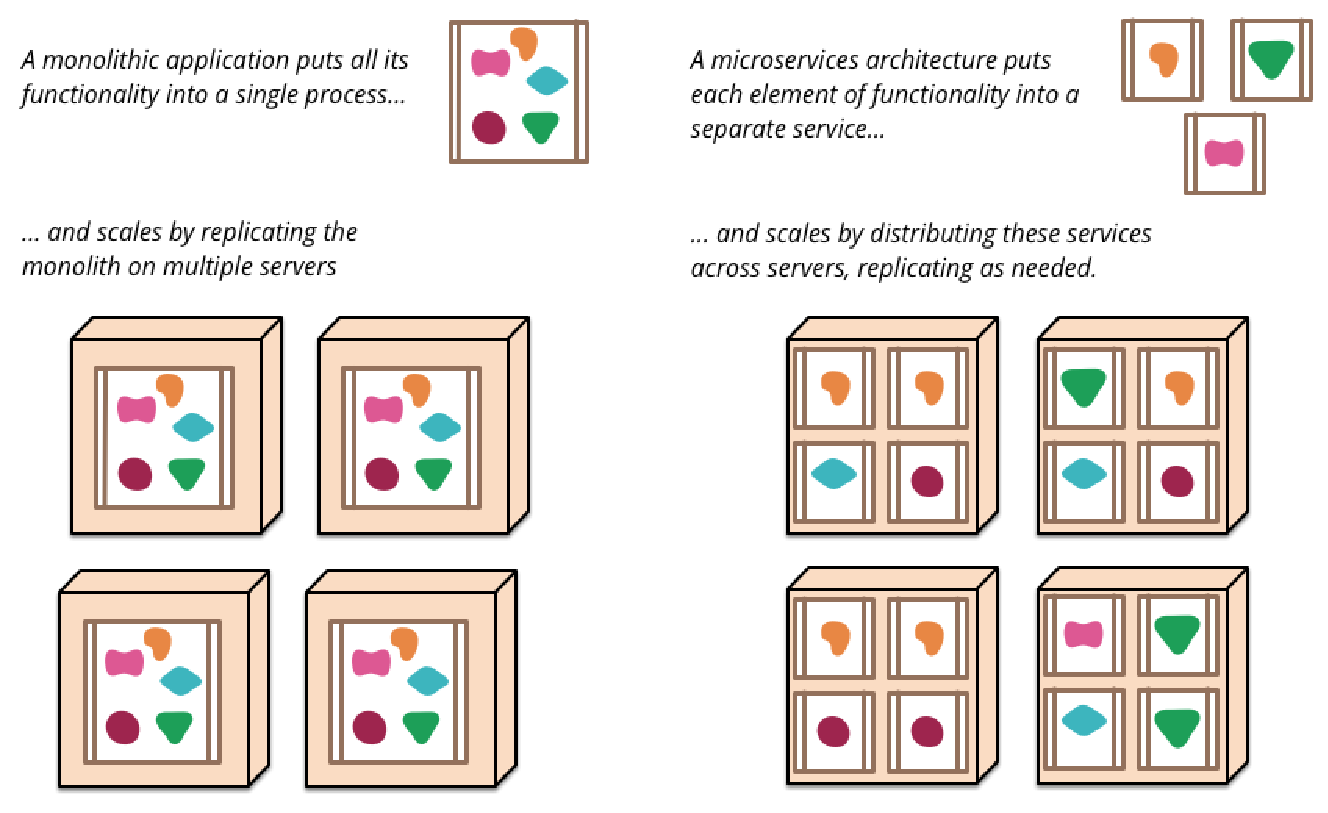
\includegraphics[width=1.00\textwidth]{monolithic_and_microservices.pdf}
    \caption{Monolithic and Microservices architectural styles\cite{microservices}.}
    \label{fig:monolithic_and_microservices}
\end{figure}

Every style presented has its owns pros and throwbacks and its usages benefit from case to case. A brief example of pros and throwbacks of each one is: for very large teams developing a big and complex service that needs to scale, its good to use the microservices architectural style, because they can tackle the problem of complexity by decomposing application into a set of manageable services which are much faster to develop by individual members, and therefore its much easier to understand and maintain, however its harder to assemble and perform the deployment of the whole service composed by tinny granular parts. In the monolithic architecture, it is normally simpler to deploy, because we  just have to copy a single packaged application to a server and run it, however when adding features to the application and it starts to grow in complexity, it gets harder to fully understand and made changes fast and correctly.

Microservices are simple enough to understand, but very hard to master in practice. Some people tend to think that microservices architecture reduce the complexity of the overall system over the monolithic architecture, however this isn't always like this. Communication is a big challenge in the realm of microservices and with a solution that integrates lots of interactions and connections throughout the whole system, the complexity starts to rise. Adding more microservices implies adding more complexity to the solution, and we have to be sure that new microservices can scale together with our existing ones.

``If you can not manage building a monolith inside a single process, what makes you think putting network in the middle is going to help?'', Simon Brown\cite{simon_brown_microservices}.

Has been said before, the implementation of a microservices architecture raises the complexity of the solution, and we need to be aware of that when we design and implement a solution based on this architectural stile. On the other side, after having the system running up, the debbug process is a lot more complex too because, instead of having a single unit to analyse, we may have hundreds or even thousands of ``micro-units'' to trace and analyse. This kind of problem takes us to an important topic, the observation and control of the system performance, taking into consideration that this system is a microservice based system.

\subsection{Observability and Controlling Performance}
\label{subsec:observability_and_controlling_performance}

Observing is ``to be or become aware of, especially through careful and directed attention; to notice''\cite{observing_definition}.

Observability is an extension of observing and its definition is the following: ``Observability is to measure of how well internal states of a system can be inferred from knowledge of its external outputs''\cite{observability}.

The presented definitions represents the meaning of the words Observing and Observability are reflected exactly as it is in the project context. For example, observe the interaction between some microservices, regarding some data resulted from their interaction, to notice a certain fault in the whole/part of the system.

Controlling in control systems is ``to manage the behaviour of a certain system''\cite{control_systems}. Controlling and Observability are dual aspects of the same problem\cite{observability}.

When we want to understand the working and behaviour of a system, we need to watch it very closely and pay special attention to all details and data it provides. This kind of details and data may be in multiple structured text formats, and it can contain lots of information regarding the interaction between microservices and the corresponding access to them. The information generated by a microservices based system is normally represented as, what we call traces and spans, presented in the next subsection \ref{subsec:traces_and_spans} - \nameref{subsec:traces_and_spans}. Therefore, we may work with this information as a starting point to perceive the characteristics of the system and build a tool that is able to be aware of it and that can perform an analysis of the data to detect some system failures.

\subsection{Distributed Tracing}
\label{subsec:distributed_tracing}



Google Dapper~\cite{Sigelman2010} 

OpenTracing~

\todo{// TODO: Write about Distributed Tracing: - Origin; - OpenTracing; - Specification; - Why; - How}

\subsection{Traces and Spans}
\label{subsec:traces_and_spans}

First things first, we can think in a trace as a group of spans. A trace is a representation of a data/execution path through the system and a span represents the logical unit of work in the system. A trace can also be a span. The span has an operation name, the start time of the operation, its duration and some annotations regarding the operation itself. An example of a span can be an \gls{http} call or a \gls{rpc} call. For a more clear insight of how spans are related with each other and with time, we have the figure \ref{fig:traces_and_spans_disposition_over_time}.

\begin{figure}[H]
    \centering
    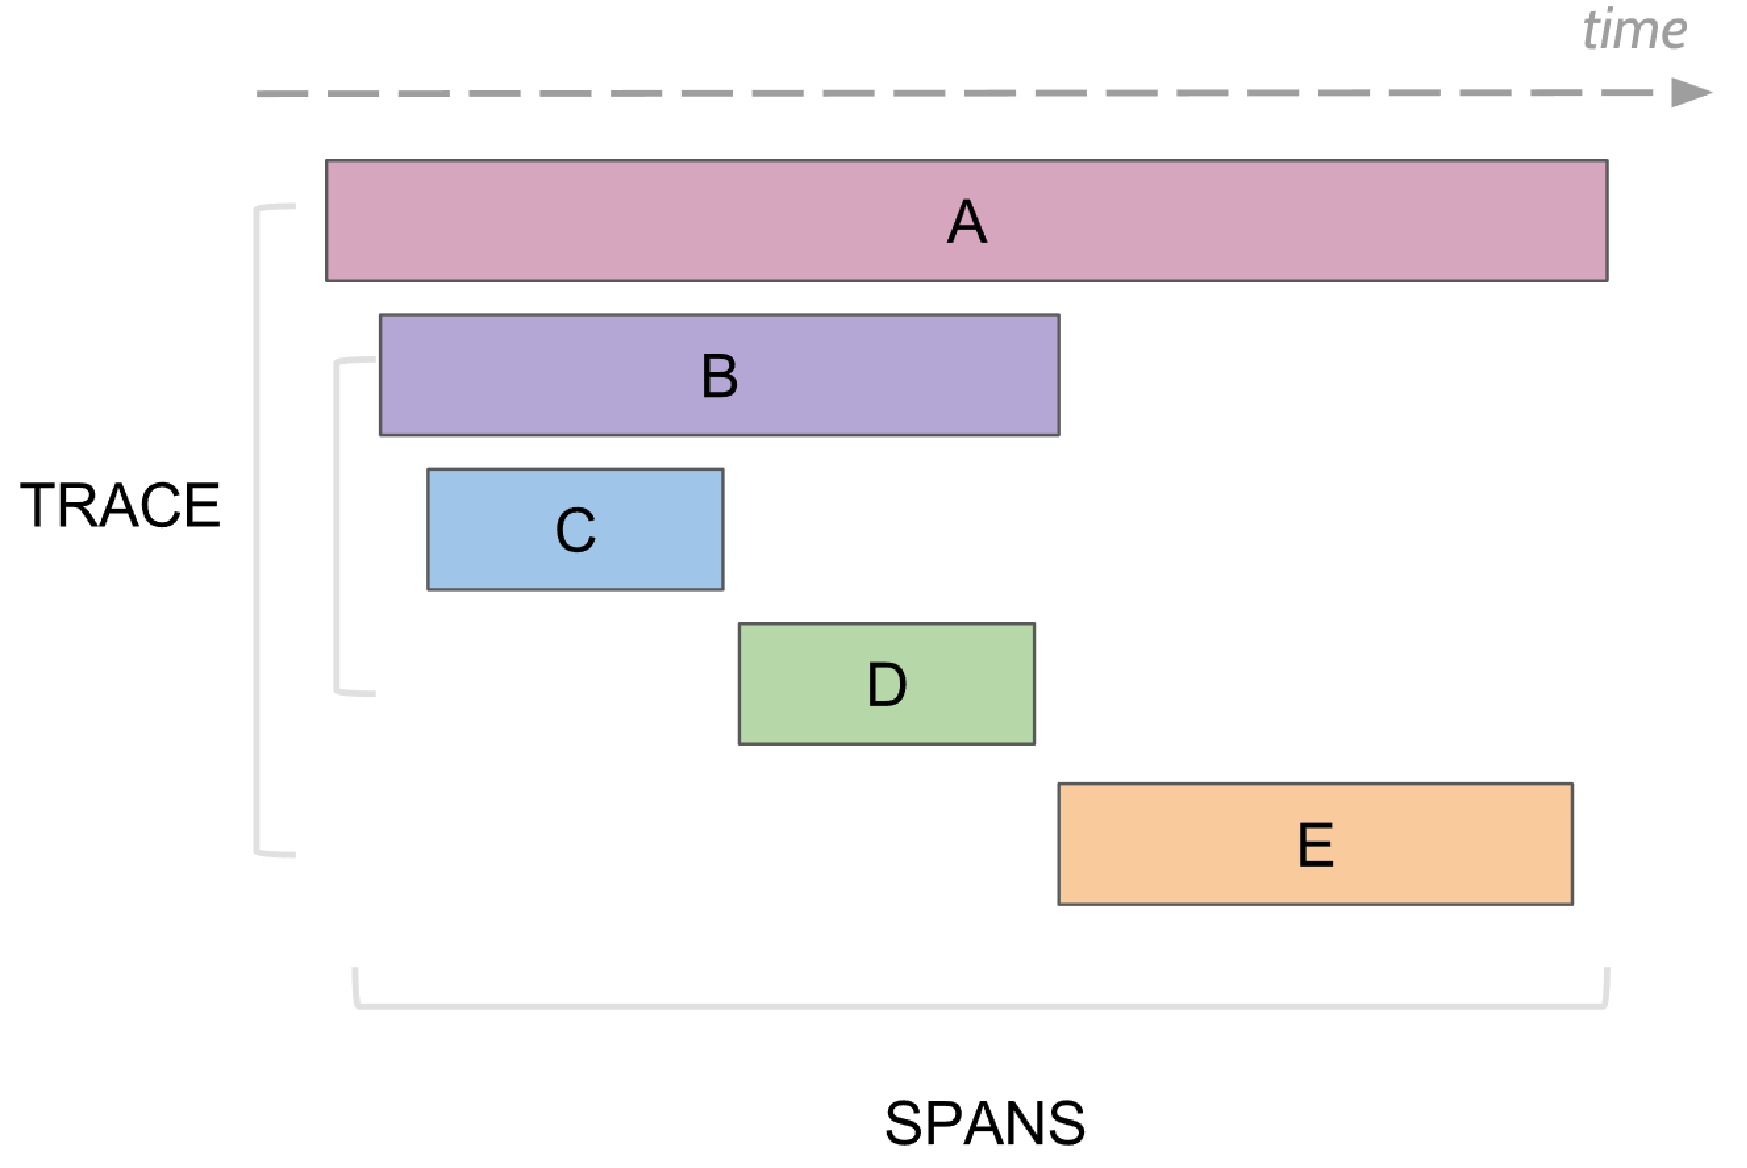
\includegraphics[width=0.60\textwidth]{traces-and-spans.pdf}
    \caption{Traces and spans disposition over time.}
    \label{fig:traces_and_spans_disposition_over_time}
\end{figure}

As we can see in the figure \ref{fig:traces_and_spans_disposition_over_time}, the spans spread over time, overlapping each other, since nothing prevents the occurrence of multiple calls in very close times. In the same figure we can see some boxes, two represent traces (box A and B) and four represent spans (boxes B, C, D and E). For a brief example, and for this case we may think of the following cases to define each operation inherent to each box: A - ``Get user info'', B - ``Fetch user data from database'', C - ``Connect to MySQL server on 127.0.0.1'(10061)'', D - ``Can't connect to MySQL server on 127.0.0.1'(10061)'' and E - ``Send error result to client''. The creators of OpenTracing have made a data model specification that says, ``with a couple of spans, we might be able to generate a span tree and model a graph of a portion of the system''\cite{open_tracing_data_model_specification}. This is because they represents causal relationships in the system. As presented by the guys who defined this specification, and again for a more clear insight, the span tree can be like the one presented in the figure \ref{fig:span_tree_example}.

\begin{figure}[H]
    \centering
    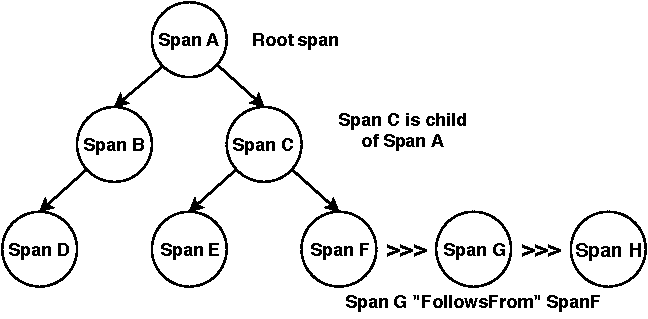
\includegraphics[width=0.80\textwidth]{span_tree_example.pdf}
    \caption{Span Tree example.}
    \label{fig:span_tree_example}
\end{figure}

In the figure \ref{fig:span_tree_example} it's represented a span tree with a trace made up of eight spans. Every span must be a child of some other span, unless it is the root span. With the information presented in the span tree, we can generate a multi-directed graph of the system (explained in the subsection \ref{subsec:graphs} - \nameref{subsec:graphs}).

This type of data is extracted and can be obtained, as trace files or by transfer protocols ex. \gls{http}, from technologies like Kubernetes\cite{what_is_kubernetes}, OpenStack\cite{what_is_opensatck}, and other cloud or distributed management system technologies that implements some kind of system or code instrumentation using, for example, OpenTracing\cite{what_is_opentracing} or OpenCensus\cite{what_is_opencensus}.

In the end and as explained before, traces and spans contains some vital system details as they are the result of instrumentation of a part or the whole system and therefore, this kind of data can be used as a starting point resource information to analyse the system.

\subsection{Graphs}
\label{subsec:graphs}

As it was briefly explained  before, we might be able to model a graph of the system using a couple of spans. ``A Graph is a set of vertices and a collection of directed edges that each connects an ordered pair of vertices'' \cite{graph_standard_definition}.

Taking the very common sense of the term, a graph is an ordered pair G = (V, E), where G is the graph itself, V are the vertices/nodes and E are the edges. The figure \ref{fig:graph_visual_representation} gives us, a simple visual representation, of what a graph really is for a more clear understanding. There we can see a graph composed by a total of five nodes that contains some labels in it and, in this case, five relationships between them.

\begin{figure}[H]
    \centering
    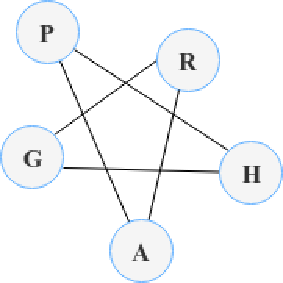
\includegraphics[width=0.30\textwidth]{images/graph_visual_representation.pdf}
    \caption{Graph visual representation.}
    \label{fig:graph_visual_representation}
\end{figure}

This graph is the representation of the following information:

V = \{'G', 'R', 'A', 'P', 'H'\}

E = \{\{'G', 'R'\}, \{'R', 'A'\}, \{'A', 'P'\}, \{'P', 'H'\}, \{'H', 'G'\}\}

There are multiple types of graphs. In this term they can be undirected, where the set of edges don't have any orientation between a pair of nodes like in this example, or be directional, where the set of edges have one and only one orientation between a pair of nodes, or be a multigraph, where in multiple edges are more than one connection between a pair of node that represents the same relationship, and so forth.

Graphs can have many use cases, has they can model the representation of a lot of real life practical problems in the fields like physics, biology, social and information systems and for the purpose of this thesis, they are considered first class citizens.

A \gls{gdb} is ``a database that uses graph structures for semantic queries with nodes, edges and properties to represent and store data''\cite{graph_database_definition}.

The composition of a \gls{gdb} is based on the mathematics graph theory, and therefore this databases uses three main components called nodes, edges, and properties. This main components are defined and explained in the following list:

\begin{itemize}
    \item Node: Are the entities in the graph. They can hold any number of attributes (key-value pairs) called properties. Nodes can be tagged with labels, representing their different roles in your domain. Node labels may also serve to attach metadata (such as index or constraint information) to certain nodes.
    \item Edge (or Relationships): provide directed, named, semantically-relevant connections between two node entities (e.g. André STUDIES\_IN \gls{dei}). A relationship always has a direction, a type, a start node, and an end node. Like a Node it can attach metadata. 
    \item Property: can be any kind of metadata attached to a certain Node or a certain Edge.
\end{itemize}

\subsection{Time Series}
\label{subsec:time_series}

\todo{Introduce Time-Series data}

A \gls{tsdb} is ``is a database optimised for time-stamped or time series data like arrays of numbers indexed by time (a date time or a date time range)''\cite{time_series_database_definition}.

This kind of databases are natively implemented using specialised database algorithms to enhance it's performance and efficiency due to the widely variance of access possible. The way this databases use to work on efficiency is to treat time as a discrete quantity rather than as a continuous mathematical dimension. Usually a \gls{tsdb} allows operations like create, enumerate, update, organise and destroy various time series entries.

The \gls{tsdb} and the \gls{gdb}, presented in this subsection and in the subsection before respectively, are at the time, the most wanted and fastest growing kind of databases due to their use cases in the trending fields of Cloud and Distributed based Systems and in the \textit{Internet of Things (IoT)}. The figure \ref{fig:fastest_growing_databases} presents the growing of this databases in the last two years. As we can see in the figure presented, the \gls{tsdb} and \gls{gdb} are distancing from the remaining databases in terms of popularity starting from the same spot in December of 2016. The predictions are that this databases will not stop increasing popularity, until this kind of systems described before start losing it too.  

\begin{figure}[H]
    \centering
    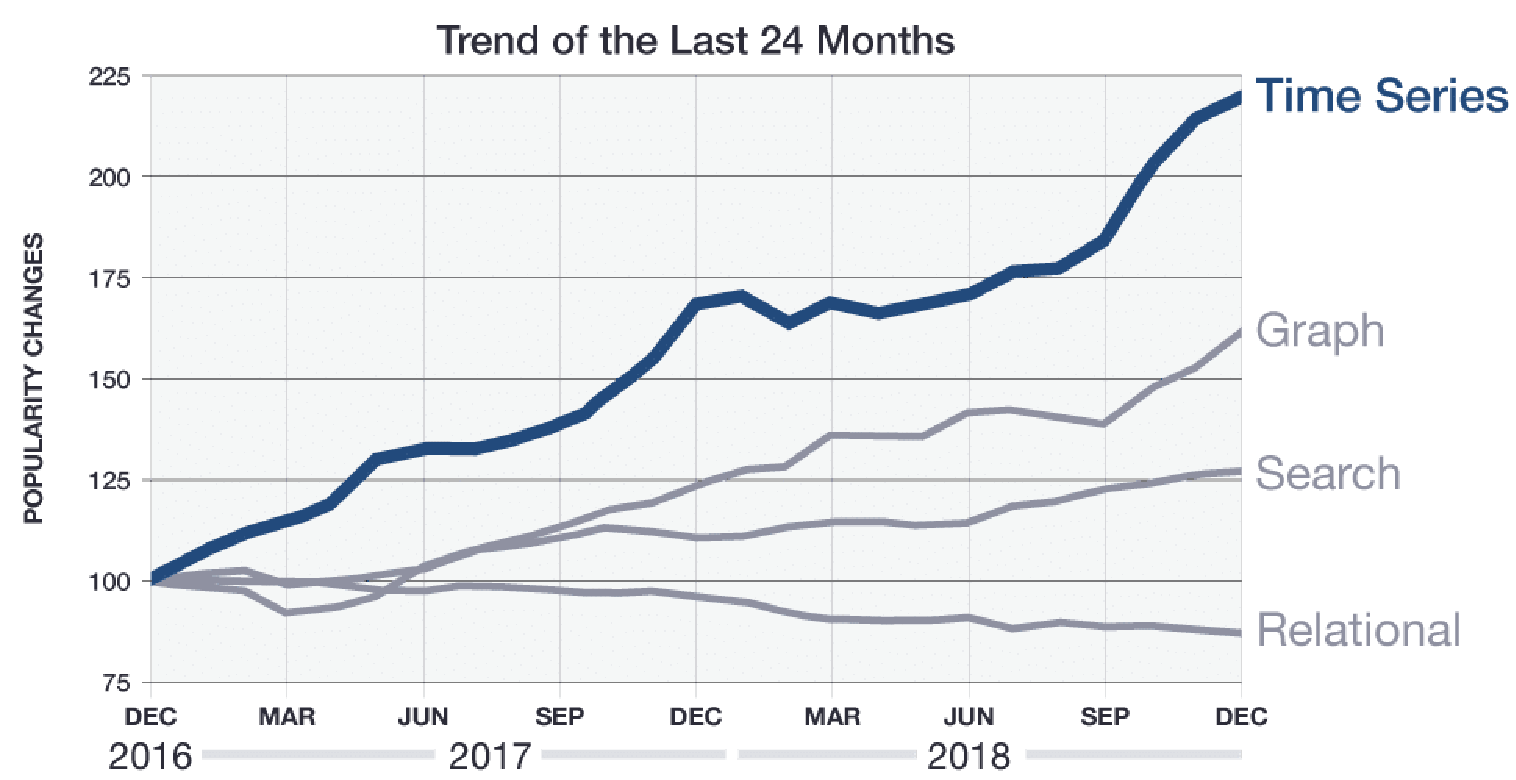
\includegraphics[width=1.0\textwidth]{images/popularity_of_time_series_databases.pdf}
    \caption{Fastest Growing Databases.\cite{time_series_databases_explained}}
    \label{fig:fastest_growing_databases}
\end{figure}

After presenting the core concepts for this work, we follow to the next section \ref{sec:related_work} - \nameref{sec:related_work} where some related work with this thesis is presented.

\section{Related Work}
\label{sec:related_work}

In this section are presented three section of the existing related work for tracing data analysis. After explaining each one, a brief reflection is made to note some directions of research for this project.

\subsection{Mastering AIOps}
\label{subsec:mastering_aiops}

\todo{// TODO: Explain what is done and how is done.}

\cite{mastering_aiops}

\subsection{Anomaly Detection using Zipkin Tracing Data}
\label{subsec:anomaly_detection_using_zipkin_tracing_data}

\todo{// TODO: Explain what is done and how is done.}

\cite{anomaly_detection_zipkin_tracing_data}

Wei Lee was contacted by email to understand better their research focus, however without success because no answer was given.

\subsection{Analyzing distributed trace data}
\label{subsec:analyzing_distributed_trace_data}

\todo{// TODO: Explain what is done and how is done.}

\cite{analysisng_distributed_trace_data}

\subsection{Research possible directions}
\label{subsec:research_possible_directions}

\todo{// TODO: Make a brief reflection about the related work.}

\section{Technologies}
\label{sec:technologies}

In this section are presented the technologies and tools that were researched, as well as the corresponding discussion considering the main objectives for this project. With the concepts presented in the section \ref{sec:concepts} in mind, the research were focused in a group of main topics regarding the problem we have in hands. The main topics were \ref{subsec:distributed_tracing_tools} - \nameref{subsec:distributed_tracing_tools}, \ref{subsec:graph_manipulation_and_processing_tools} - \nameref{subsec:graph_manipulation_and_processing_tools}, \ref{subsec:graph_database_tools} - \nameref{subsec:graph_database_tools} and \ref{subsec:time_series_database_tools} - \nameref{subsec:time_series_database_tools}.

\subsection{Distributed Tracing Tools}
\label{subsec:distributed_tracing_tools}

This sub-section presents what are the most used and known distributed tracing tools. This tools are mainly oriented for tracing distributed systems like microservices-based distributed systems. What they do is to fetch or receive trace data from this kind of complex systems, treat the information, and then present it to the user using charts and diagrams in order to explore the data in a more human-readable way. One of the best features presented in this tools is the possibility to perform queries on the tracing (e.g. by trace id and by time-frame). The table \ref{table:tracing_tools} presents the most well-known OpenSource tracing tools.

\begin{table}[H]
\caption{Tracing tools comparison.}
\label{table:tracing_tools}
\centering
\large
\begin{tabularx}{\linewidth} {
    |>{\hsize=0.70\hsize}X| 
     >{\hsize=1.15\hsize}X|
     >{\hsize=1.15\hsize}X| }
     \hline
    \textbf{Name} 
    & Jaeger
    & Zipkin \\ \hline
    \textbf{Repository}
    & Jaeger GitHub \cite{jaeger_github}
    & Zipkin GitHub \cite{zipkin_github} \\ \hline
    \textbf{Brief description}
    & It is a distributed tracing and monitoring system released as open source by Uber Technologies, that is used for monitoring and troubleshooting microservices-based distributed systems.
    & It is a distributed tracing and monitoring system. It helps gather timing data needed to troubleshoot latency problems in microservice architectures. It manages both the collection and lookup of this data. Zipkin’s design is based on the Google Dapper paper. \\ \hline
    \textbf{Pros}
    & OpenSource. \newline
    Docker-ready. \newline
    Can be used with some Zipkin functionalities, as it has a collector dedicated to it. \newline
    Dynamic sampling rate. \newline
    Browser UI.
    & OpenSource. \newline
    Docker-ready. \newline
    Allows lots of span transport ways (HTTP, Kafka, Scribe, AMQP). \newline
    Browser UI. \\ \hline
    \textbf{Cons} 
    & Only supports two span transport ways (UDP and HTTP).
    & Fixed sampling rate. \\ \hline
    \textbf{Used mainly by}
    & Uber
    & Lightstep \\ \hline
\end{tabularx}
\end{table}

As we can see, this kind of tools are very similar and very good for monitoring and tracing a system as they provide a bunch of pros like being open source, containerized, support for some well known technologies for span transport and aggregate the spans in a good representational browser user-interface. However they are always focused on span and trace lookup and presentation, and do not provide a more interesting analysis of the system, for example to determine if there is any problem related to some microservice presented in the system. This kind of work falls into the user (\gls{devops}) and he needs to perform the investigation and analyse the traces and spans with the objective of find anything wrong with them.

This kind of tools can be a good starting point for the problem that we face, because they already do some work for us like grouping the data generated by the system and provide some way to visualize it. 

\subsection{Graph Manipulation and Processing Tools}
\label{subsec:graph_manipulation_and_processing_tools}

Considering that we have data to be processed and manipulated, we have to be sure that we can handle it for analysis. For this purpose, and knowing that the data is a representation and an abstraction of a graph, we needed to study the frameworks available this task. The table \ref{table:graph_manipulation_and_processing_tools_comparison} presents the main technologies available at the time for graph manipulation and processing.

\begin{table}[H]
\caption{Graph manipulation and processing tools comparison.}
\label{table:graph_manipulation_and_processing_tools_comparison}
\centering
\large
\begin{tabularx}{\linewidth} {
    |>{\hsize=0.7\hsize}X| 
     >{\hsize=1.1\hsize}X|
     >{\hsize=1.1\hsize}X| 
     >{\hsize=1.1\hsize}X| }
\hline
\textbf{Name} 
& Apache Giraph \cite{apache_giraph}
& Ligra \cite{ligra_graph_processing_framework}
& NetworkX \cite{networkx} \\ \hline
\textbf{Description}
& It's an iterative graph processing system built for high scalability. For example, it is currently used at Facebook to analyse the social graph formed by users and their connections.
& A library collection for graph creation and manipulation, and for analysing networks. 
& A Python package for the creation, manipulation, and study of the structure, dynamics, and functions of complex networks. \\ \hline
\textbf{Licence}\cite{software_license}
& Free Apache 2
& MIT
& BSD - New License \\ \hline
\textbf{Supported languages} 
& Java and Scala.
& C and C++. 
& Python. \\ \hline
\textbf{Pros} 
& Distributed and very scalable. \newline
Excellent performance (Can process one trillion edges using 200 modest machines in 4 minutes).
& Can handle very large graphs. \newline
Exploit large memory and multi-core \gls{cpu}'s (Vertically scalable).
& Good support and very easy to install with Python. \newline
Lots of graph algorithms already implemented and tested. \newline
Mature project.\\ \hline
\textbf{Cons} 
& Uses the ``Think-Like-a-Vertex'' programming model that often forces into using sub-optimal algorithms and is quite limited and sacrifices performance for scaling out. \newline
Can't perform many complex graph analysis tasks because it primarily supports Bulk synchronous parallel.
& Lack of documentation and therefore, very hard to use. \newline
Don't have many usage in the community.
& Not scalable (single-machine). \newline
High learning curve due to the maturity of the project. \newline
Begins to slow down when there's a high amount of data (400.000 plus nodes). \\ \hline
\end{tabularx}
\end{table}

With the information presented in the previous table, we can have a notion that this three frameworks don't work and perform in the same level in many ways. 

One thing to consider when comparing them is the scalability and performance that each can provide, for instance, in this component the first one, Apache Giraph is the winner since it is implemented with the distributed systems paradigm in mind and can scale to multiple-machines to get the job done in no time, considering high amounts of data. In other way, we have the third framework, called NetworkX, that is different from the previous as it works in a single-machine and doesn't have the ability to scale to multiple-machines. This can be a very problematic feature if we are dealing with very high amounts of data and we have to process it in short amounts of time. The last framework, called Ligra, works in a single-machine environment like the previous one, but it can scale vertically as it has the benefit of use and exploit multi-core \gls{cpu}'s. 

The second, and also most important thing to consider, is the support and quantity of implemented graph algorithms in the framework, and in this field the tables turned, and the NetworkX has a lot of advantage as it have lots of implemented graph algorithms defined and studied in graph and networking theory. The remaining frameworks don't have very support either because they don't have it documented or because the implementation and architecture that where considered don't allow to implement it.

For a more clear insight of the position of the presented technologies in the previous table, we have the figure \ref{fig:graph_manipulation_and_performance_tools_diagram_comparison} \cite{graph_data_management_systems}.

\begin{figure}[H]
    \centering
    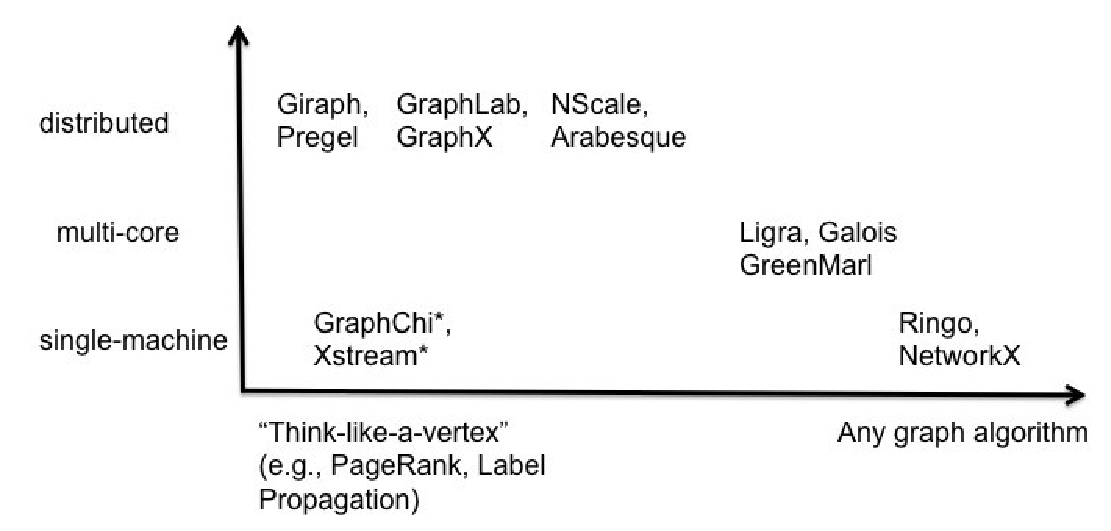
\includegraphics[width=0.80\textwidth]{images/graph_manipulation_tools_diagram_comparison.pdf}
    \caption{Graph manipulation tools comparison, regarding scalability and graph algorithms.}
    \label{fig:graph_manipulation_and_performance_tools_diagram_comparison}
\end{figure}

With the presented figure, our perception of what we might choose when considering this tools is more clear, but we have always some trade offs we cannot avoid. The best approach, and if it's possible, is to consider the usage of an hybrid environment where Giraph and NetworkX coexist one with another, as one fills the gaps of the other, but always taking into consideration that a bottleneck will occur between them \cite{graph_frameworks_performance_evaluation} and that there are almost none implementation where they coexist \cite{graph_frameworks_performance_evaluation} because of their disparity.

\subsection{Graph Database Tools}
\label{subsec:graph_database_tools}

Manipulating and process graph data is not enough, we need to store this data somewhere, and to do this we need a \gls{gdb}. The results of the research for the best graph databases tools available are presented in the table \ref{table:graph_databases_comparison}.

\begin{table}[!b]
\caption{Graph databases comparison.}
\label{table:graph_databases_comparison}
\centering
\large
\begin{tabularx}{\linewidth} {
    |>{\hsize=0.7\hsize}X| 
     >{\hsize=1.1\hsize}X|
     >{\hsize=1.1\hsize}X| 
     >{\hsize=1.1\hsize}X| }
    \hline
    \textbf{Name} 
    & ArangoDB \cite{arangodb_documentation}
    & Facebook TAO \cite{facebook_tao_article}
    & Neo4J \cite{neo4j_documentation} \\ \hline
    \textbf{Description} 
    & It's a NoSQL database developed by ArangoDB Inc. that uses a proper query language to access the database.
    & TAO, “The Associations and Objects”, is a proprietary database, developed by Facebook, that stores all the data related to the users in the social network. 
    & It's the most popular open source graph database. Has been developed by Neo4J Inc. and is completely open to the community. \\ \hline
    \textbf{Licence}
    & Free Apache 2 
    & Proprietary 
    & GPLv3 CE \\ \hline
    \textbf{Supported languages} 
    & C++ \newline 
    Go \newline
    Java \newline
    JavaScript \newline
    Python \newline
    Scala
    & \centering -----
    & Java \newline
    JavaScript \newline
    Python \newline
    Scala \\ \hline
    \textbf{Pros} 
    & Multi data-type support (key/value, documents, graphs). Allows the combination of different data access patterns in a single query. Supports cluster deployment. 
    & Very fast(~=100ms latency). Accepts millions of calls per second. Distributed.
    & Supports ACID(Atomicity, Consistency, Isolation, Durability)\cite{acid_definition}. High-availability. Has a visual node-link graph explorer. REST \gls{api} interface. Most popular open source graph database. \\ \hline
    \textbf{Cons} 
    & Needed to learn a new query language called AQL(Arango Query Language). High learning curve. Has paid version with high price tag.
    & Not accessible to use.
    & Can’t be distributed (It needs to be vertically scaled). \\ \hline
\end{tabularx}
\end{table}

As we can notice by the data provided by the presented table, the state of the art about graph databases is not very good. The offers are very limited and all of them lack something when we start to see them in detail. The interest in this databases is increasing as graph technology tend to have many use cases and solve lots of problems nowadays.

Facebook detains the most powerful and robust system for this purpose, but as it is the base of their business because they need to perform large operations in their huge social graph in reduced times, it is a proprietary technology and is only referenced in some articles \cite{facebook_tao_article}.

The remaining two tools, are very supported by the community because of their license and demand, however based on the stars and forks of their repositories, Neo4J is more well received by the community and tends to become more popular. It doesn't implement horizontal scalability by design and this can be a risk when using it in systems with scalabilty in mind, but there are some authors that report they were able to perform implementations and surpass the scalability issue, however with many snags\cite{neo4j_scalable}. ArangoDB supports scalability by default as we can see in the figure \ref{fig:arangodb_vs_neo4j_scalability}\cite{arangodb_vs_ne4j}, but it has a very hard query language with a high learning curve inherent to it, and it is payed to use some special features like SmartGraphs storage\cite{arangodb_smart_graphs} that improves the writing of graph in distributed databases.

\begin{figure}[H]
    \centering
    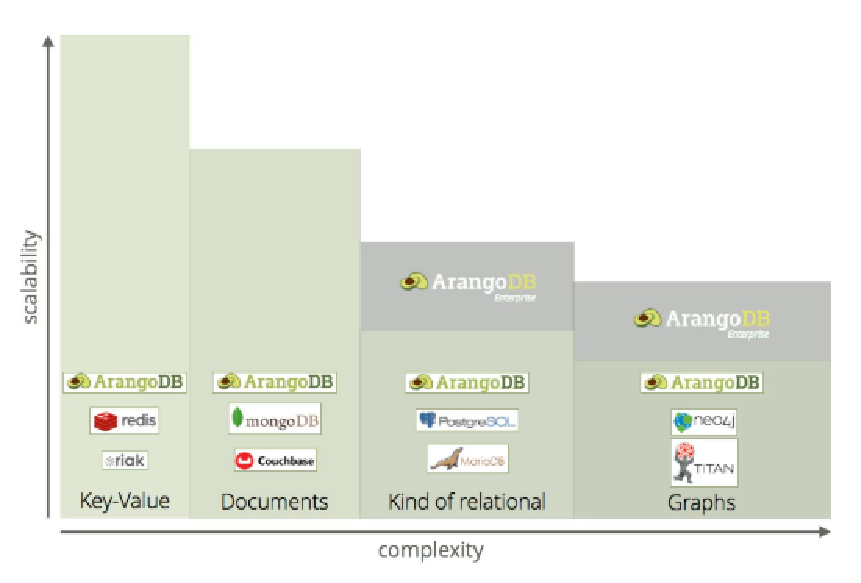
\includegraphics[width=0.80\textwidth]{images/arangodb_vs_neo4j_scalability.pdf}
    \caption{ArangoDB vs. Neo4J scalability over complexity.}
    \label{fig:arangodb_vs_neo4j_scalability}
\end{figure}

\subsection{Time-Series Database Tools}
\label{subsec:time_series_database_tools}

As we intend to extract useful data from span trees and graphs, we need to store it somewhere. We already know that the spans and trace data are directly related with time based information, explained in the subsection \ref{subsec:traces_and_spans} - \nameref{subsec:traces_and_spans}, so the best way to store the gathered or calculated information from them is in a \gls{tsdb}.

The figure \ref{fig:time_series_databases_ranking} present the ranking of the \gls{tsdb} at the current time\cite{tsdb_ranking}.

\begin{figure}[h!]
    \centering
    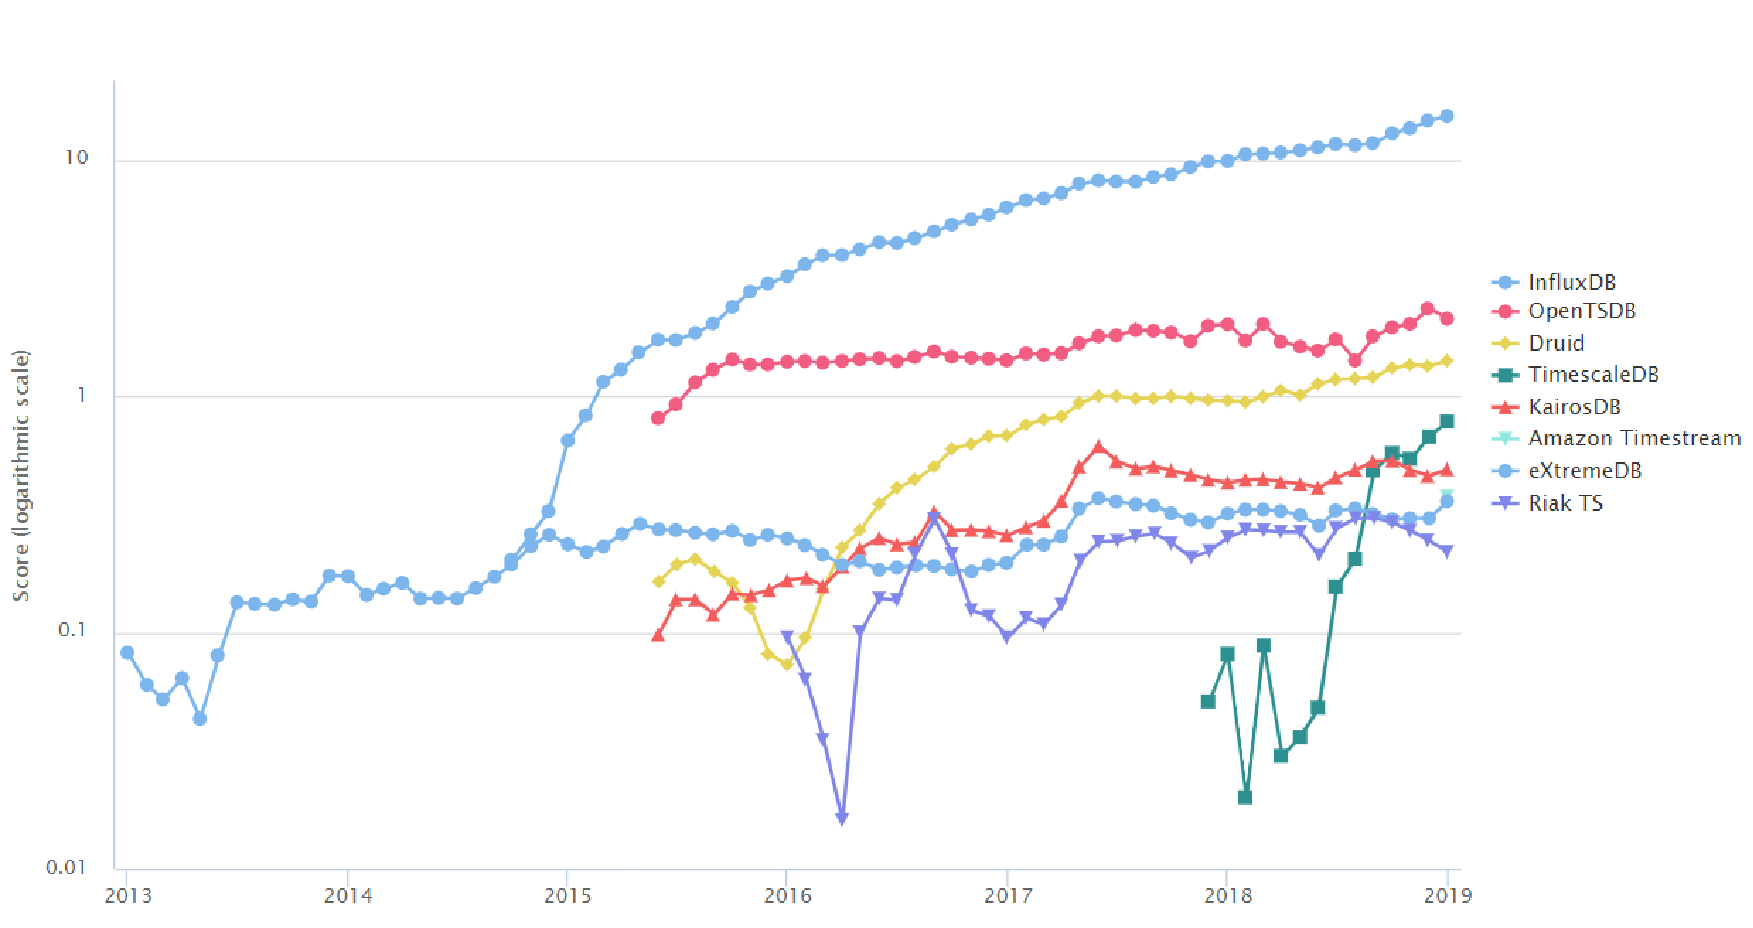
\includegraphics[width=1.00\textwidth]{images/time_series_databases_ranking.pdf}
    \caption{\gls{tsdb}s ranking from 2013 to 2019.}
    \label{fig:time_series_databases_ranking}
\end{figure}

The table \ref{table:time_series_databases_comparison} exposes a comparison between the two top databases presented in the ranking, the \textit{InfluxDb} and \textit{OpenTSDB}, two very well known databases in the world of \gls{tsdb}, in order to understand the advantages and disadvantages of each one.

\begin{table}[H]
\caption{Time-series databases comparison.}
\label{table:time_series_databases_comparison}
\centering
\large
\begin{tabularx}{\linewidth} {
    |>{\hsize=0.50\hsize}X| 
     >{\hsize=1.25\hsize}X|
     >{\hsize=1.25\hsize}X| }
    \hline
    \textbf{Name} 
    & InfluxDB \cite{influxdb}
    & OpenTSDB \cite{opentsdb} \\ \hline
    \textbf{Description} 
    & It is an open-source time series database developed by InfluxData written in Go and optimised for fast, high-availability storage and retrieval of time series data in fields such as operations monitoring, application metrics, Internet of Things sensor data, and real-time analytics.
    & It is a distributed, scalable Time Series Database (TSDB) written on top of HBase. OpenTSDB was written to address a common need: store, index and serve metrics collected from computer systems (network gear, operating systems, applications) at a large scale, and make this data easily accessible and graphable. \\ \hline
    \textbf{Licence}
    & MIT 
    & GPL \\ \hline
    \textbf{Supported languages} 
    & Erlang \newline
    Go \newline
    Java \newline
    JavaScript \newline
    Lisp \newline
    Python \newline
    R \newline
    Scala
    & Erlang \newline
    Go \newline
    Java \newline
    Python \newline
    R \newline
    Ruby \\ \hline
    \textbf{Pros} 
    & Scalable in the enterprise version. \newline
    Outstanding high performance. \newline
    Accepts data via HTTP, TCP, and UDP protocols. \newline
    SQL like query language. \newline
    Allows real-time analytics.
    & It's massively scalable. \newline
    Great for large amounts of time-based events or logs. \newline
    Accepst data via HTTP and TCP access protocols. \newline
    Good platform for future analytical research into particular aggregations on event/log data. \newline
    Doesn't have paid version. \\ \hline
    \textbf{Cons} 
    & Enterprise high price tag. \newline
    Clustering support only available in the enterprise version.
    & Expensive to try. \newline
    Not a good choice for general-purpose application data. \\ \hline
\end{tabularx}
\end{table}

Based on the information presented in the referenced table, we can notice that this two databases are very similar on what they offer like the access protocols and scalability capabilities. In the point of licence, both are open source, however the first one, InfluxDB, has an enterprise paid version that is not very well exposed in its documentations and much people don't even notice it, contrarily to OpenTSDB which is completely free. The enterprise version of InfluxDB provides clustering support, high availability and scalability\cite{influxdb_vs_opentsdb}, features that OpenTSDB offer for free, however in terms of performance, InfluxDB outperforms OpenTSDB in almost every benchmark by a far distance as we can see in the figures \ref{fig:influxdb_vs_opentsdb_write_throughput} and \ref{fig:influxdb_vs_opentsdb_storage_requirements}.

\begin{figure}[H]
    \centering
    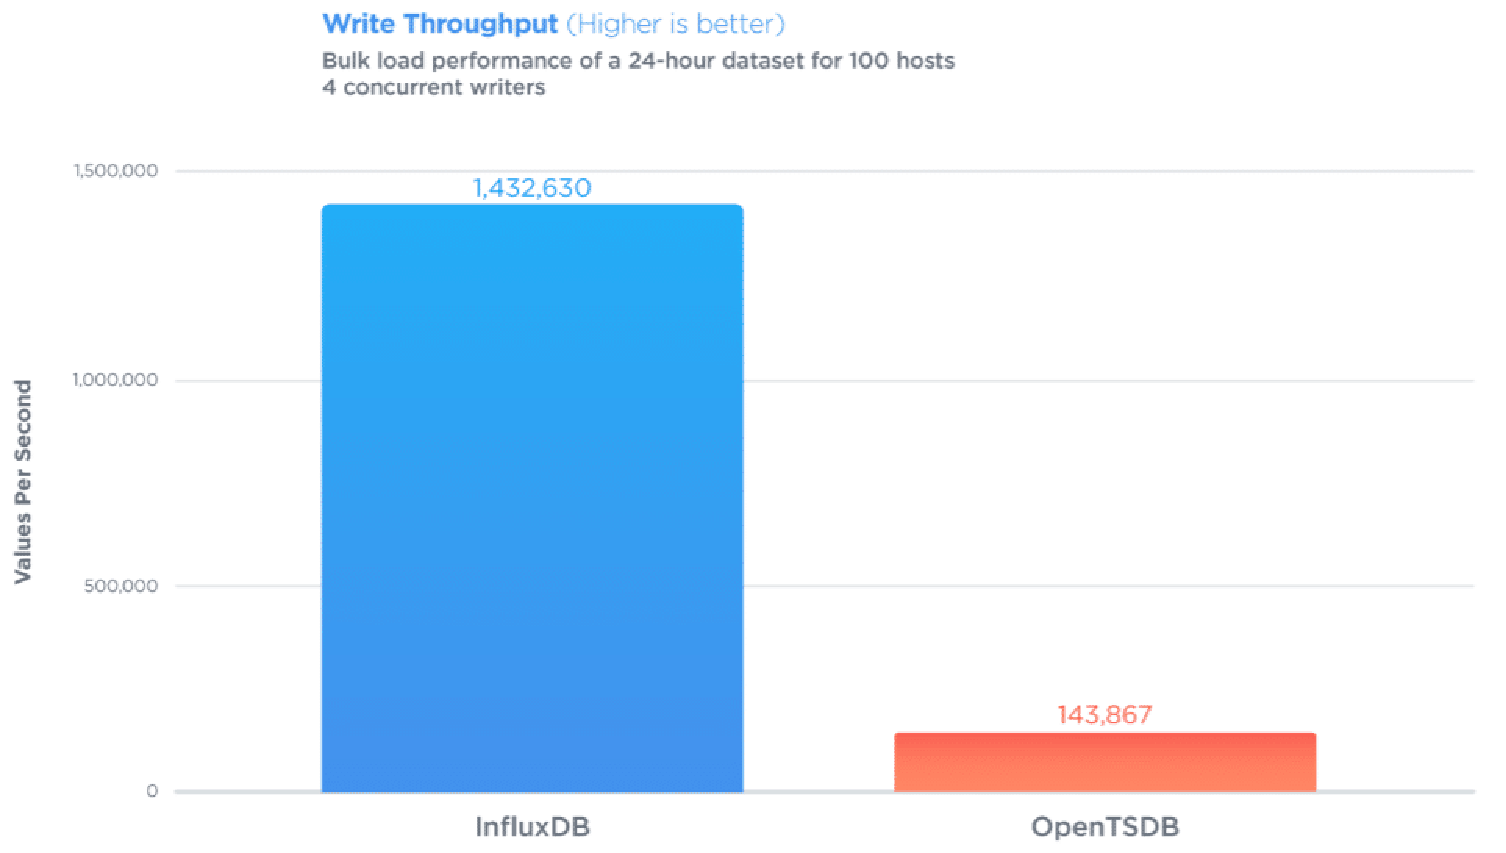
\includegraphics[width=1.00\textwidth]{images/influxdb_vs_opentsdb_write_throughput.pdf}
    \caption{InfluxDB vs OpenTSDB write throughput performance\cite{influxdb_vs_opentsdb}.}
    \label{fig:influxdb_vs_opentsdb_write_throughput}
\end{figure}

\begin{figure}[H]
    \centering
    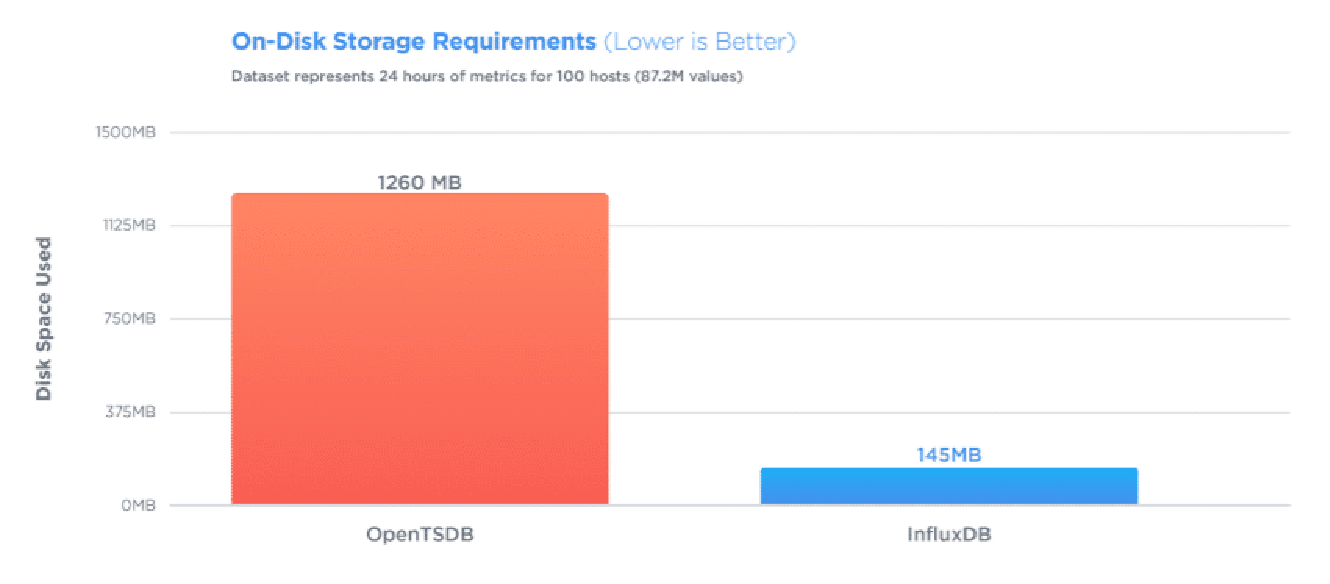
\includegraphics[width=1.00\textwidth]{images/influxdb_vs_opentsdb_storage_requirements.pdf}
    \caption{InfluxDB vs OpenTSDB storage requirements\cite{influxdb_vs_opentsdb}.}
    \label{fig:influxdb_vs_opentsdb_storage_requirements}
\end{figure}

After providing the state of the art involved with this work to the reader in this chapter, the document flows to the next chapter \ref{chap:research_objectives_and_approach} - \nameref{chap:research_objectives_and_approach}, where the objectives of this research and the approach taken to each component of work are presented and discussed.

%-------------------------------------------------------------------------------------------------
\checkoddpage
\ifthenelse{\boolean{oddpage}}
{ % Odd page
\newpage
\blankpage}
{ % Even page
}
%-------------------------------------------------------------------------------------------------